\section{Experimental results}\sloppy
\label{sec:exp}

  % Here you evaluate your work using experiments. You start again with a
  % very short summary of the section. The typical structure follows.
  %
  % \mypar{Experimental setup} Specify the platform (processor, frequency, maybe OS, maybe cache sizes)
  % as well as the compiler, version, and flags used. If your work is about performance, 
  % I strongly recommend that you play with optimization flags and consider also icc for additional potential speedup.
  %
  % Then explain what kind of benchmarks you ran. The idea is to give enough information so the experiments are reproducible by somebody else on his or her code.
  % For sorting you would talk about the input sizes. For a tool that performs NUMA optimization, you would specify the programs you ran.

\mypar{Experimental setup}
Benchmarks were run on two distinct setups: a node of ETH's Euler cluster, a convential x86 multicore platform, and on ETH's Einstein machine with ssh-access to a Knight's Corner Intel Xeon Phi coprocessor. An Euler node consists of two Intel Xeon E5-2697v2 processors for a total of 24 x86 cores in a dual-socket NUMA setup. The x86 benchmark code was compiled with GCC 4.9.2 with OpenMP 4.0, while the Xeon Phi host code was compiled with GCC 4.8.2. Both setups used precompiled TBB 4.4 for
parallelization. The Xeon
Phi setup additionally uses the MPI library from Intel Parallel Studio XE 2016 when communicating with the Xeon Phi on both host and coprocessor, and the MIC code (\texttt{-mmic}) is compiled using ICC 15.0.0. All code was compiled with \texttt{-std=c++11} standard, \texttt{-O3} optimization and \texttt{-march=native} SIMD vectorization for both GCC and ICC. In particular computing Euclidian distances between high-dimensional input offers a potential gain of
vectorization. 

\mypar{Data set}
Measurements are done on the TEXMEX~\cite{jegou2011} data set, which is a collection of SIFT~\cite{lowe1999a,lowe2004a} descriptors: 128-dimensional vectors invariantly describing features in images, commonly used in computer vision to recognize transformations between images taken of the same underlying content. The data set is produced specifically by the authors of~\cite{jegou2011} to test the performance of nearest neighbor algorithms, as it offers a high input size of
high-dimensional data applied to a common real world problem. Results presented below are run for the data set containing one million reference points queried with ten thousand test points with $k=100$.  

  % \mypar{Results}
  % Next divide the experiments into classes, one paragraph for each. In each class of experiments you typically pursue one questions that then is answered by a suitable plot or plots. For example, first you may want to investigate the performance behavior with changing input size, then how your code compares to external benchmarks.
  %
  % For some tips on benchmarking including how to create a decent viewgraph see pages 22--27 in \cite{Pueschel:10}.
  %
  % {\bf Comments:}
  % \begin{itemize}
  %   \item Create very readable, attractive plots (do 1 column, not 2 column plots
  %     for this report) with readable font size. However, the font size should also not be too large; typically it is smaller than the text font size.
  %     An example is in Fig.~\ref{fftperf} (of course you can have a different style).
  %   \item Every plot answers a question. You state this question and extract the
  %     answer from the plot in its discussion.
  %   \item Every plot should be referenced and discussed.
  % \end{itemize}
  %
  % \begin{figure}\centering
  %   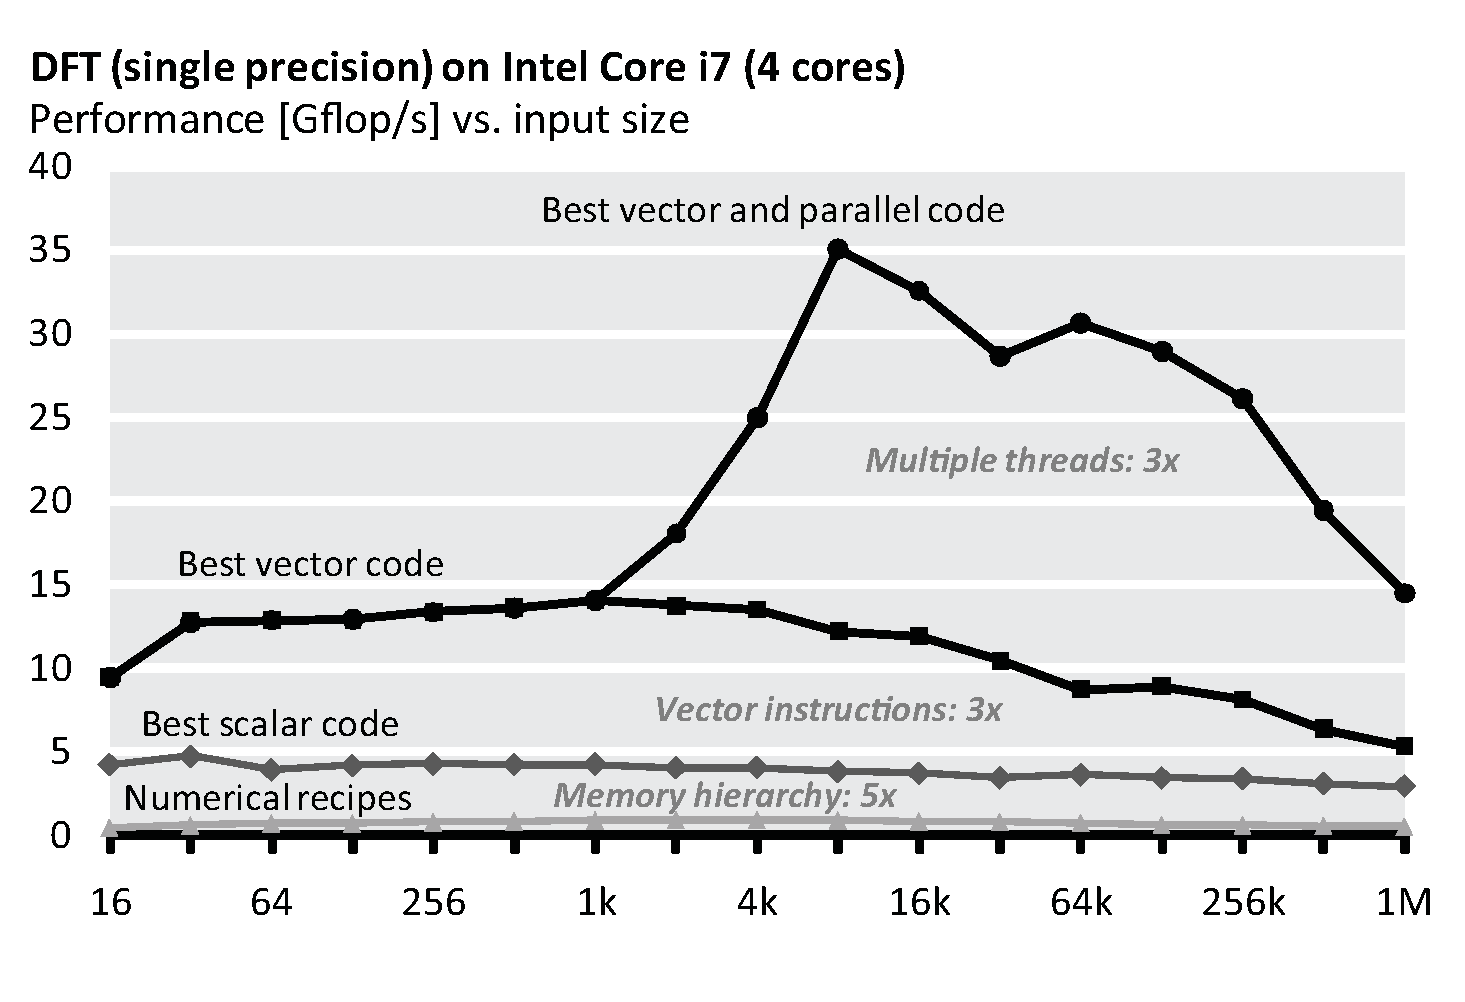
\includegraphics[scale=0.33]{./03_results/figs/dft-performance.eps}
  %   \caption{Performance of four single precision implementations of the
  %   discrete Fourier transform. The operations count is roughly the
  %   same. The labels in this plot are maybe a little bit too small.\label{fftperf}}
  % \end{figure}

\mypar{Build performance} To evaluate the performance of the build parallelization scheme described in Section~\ref{sec:method}, an implementation is compared against the implementation provided by the FLANN library. Because FLANN implements no parallelization of the tree build, including the trivial parallelization of building $N$ randomized trees in parallel, the implementation described here must scale beyond $N$ processors to demonstrate the advantage of the recursive task
spawning scheme. This work contains no demonstration of the suggested parallel build scheme run on Xeon Phi, as compiling the code with ICC for unknown reasons resulted in a build time two orders of magnitude higher than when compiled with GCC even on the host platform.

\mypar{Search performance} Since no novel work is done to improve over the search algorithm implemented for randomized k-d trees in the FLANN library, the performance of the implementation presented here is only expected to match that of FLANN. The contribution of this work is to evaluate the performance of the search algorithm on the Xeon Phi platform, whose architecture is expected to be a good match to the randomized k-d tree search due to several factors: firstly the highly parallel nature of the search offers full
hardware utilization when queried with a sufficiently high numbers of points, while not being fully vectorizable due to the heterogeneousness of the tree structure. Secondly, the algorithm offers benefits of sharing memory between caches without causing performance hits due to writes. Thirdly, computing the Euclidian distance between high dimensional input offers an opportunity to take advantage of the 512-bit wide SIMD units on the Knight's Corner cores, treating up to 16
single precision floating point numbers in parallel. 
Because of the issues with the build algorithm compiled with ICC as described above, search on the Xeon Phi is done by building the randomized trees on the host processor, then transferring this using explicit MPI send and receive calls. This allows the host and coprocessor binaries to be built and linked separately with different compilers, relying on Intel's MPI library for interfacing.


  % mainfile: ./../report.tex
